% !TEX program = xelatex
\documentclass[a4paper]{article}
\usepackage{amsmath}
\usepackage{amsthm}
\usepackage[left=1.8cm,right=1.8cm,top=2.2cm,bottom=2.0cm]{geometry}
\usepackage{ctex}
\usepackage{enumerate}
\usepackage{fancyhdr}
\usepackage{xpatch}
\usepackage{graphicx} 
\usepackage{float} 
\usepackage{subfigure} 
\usepackage{amsfonts}
\usepackage{mathtools}
\usepackage{framed}
\usepackage{multicol}
\usepackage{listings}
\usepackage{hyperref}
\usepackage{tikz}
\usetikzlibrary{automata,positioning}
\theoremstyle{definition}
\newtheorem*{solution*}{\textbf{Solution:}}
\newtheorem*{proof*}{\textbf{Proof:}}
\newtheorem{theorem}{Theorem}[subsection]
\newtheorem{definition}{Definition}[subsection]
\newtheorem{lemma}{Lemma}[subsection]
\makeatletter

\AtBeginDocument{\xpatchcmd{\@thm}{\thm@headpunct{.}}{\thm@headpunct{}}{}{}}
\makeatother

\pagestyle{fancy}
\renewcommand{\baselinestretch}{1.15}

\usepackage{paralist}
\let\itemize\compactitem
\let\enditemize\endcompactitem
\let\enumerate\compactenum
\let\endenumerate\endcompactenum
\let\description\compactdesc
\let\enddescription\endcompactdesc

% shorten footnote rule
\xpatchcmd\footnoterule
  {.4\columnwidth}
  {1in}
  {}{\fail}

\title{CS 131 Compilers: Discussion 8: Scope \& Type Inference and Unification}
\author{\textbf{杨易为}~~\textbf{季杨彪}~~\textbf{尤存翰} \\ \texttt{ \{yangyw,jiyb,youch\}@shanghaitech.edu.cn}}


\begin{document}
\maketitle
\section{Scope}
Whenever a scope is introduced, the compiler gives it a name and puts it in a structure (a tree) that makes it easy to determine the position of that scope in relation to other scopes, and it is marked as being the current scope. When a variable is declared, its assigned to the current scope.

Four kinds of scopes and their life cycle in python: 
\begin{enumerate}
    \item local (local scope), that is, the temporary variables defined in the function, when the function ends, the life cycle of the variables ends. 
    \item enclosed (closure, the local scope of the nested parent function), that is, the local variables of the outer function of the closure, the end of the outer function, the end of the life cycle of the variable.
    \item global (global variables), that is, variables defined at the module level, the module is destroyed, the life cycle of the variable will end. 
    \item bulit-in (built-in function) is a variable built in python interpreter, virtual machine. The order of searching variables is: (1) -> (2) -> (3) -> (4)
\end{enumerate}

\begin{enumerate}
\begin{lstlisting}[language=python}]
a = 10
def func():
  a = 20
  print(a)
func()
print(a)
"""
Output:
20
10
"""
\end{lstlisting}

\begin{lstlisting}[language=python]
    a = 10
    def func():
      a = 20
        global a  # IndentationError: unindent does not match any outer indentation level
      print a
    func()
    print a
\end{lstlisting}
\end{enumerate}
\section{Mid Term preparation}
\subsection{Regular Expressions}
\begin{enumerate}
   \item Write a regex that matches binary strings divisible by 8.
   \item Provide aregulargrammar for the regex from part (a).
 \end{enumerate}

  \subsection{Finite State Automata}
  \begin{enumerate}
    \item Write the corresponding NFA for the regular expression $(0|1)?(10|01)+$;
    \item Convert the NFA from part (a) into a DFA.
  \end{enumerate}
  
  \subsection{Grammar Rewriting and LL(k) Parsing}
  $$
\begin{aligned}
&\begin{aligned}
S &: E \dashv \\
E: & E+E \\
& \mid E * E
\end{aligned}\\
&\quad 
 \ \mid \text { ID }
\end{aligned}
$$
  \begin{enumerate}
    \item Show that the grammar is ambiguous with two different leftmost derivations of the string $a+b*c$;
    \item Rewrite this grammar so that it preserves the standard order of operations, is LL(1),and is unambiguous.  Draw the resulting tree for the string $a+b*c$;
    \item Write down the equivalent unambiguous grammar that enforces both left associativity and correct precedence.  Why can’t this be achieved with an LL(1) grammar?
  \end{enumerate}

  \subsection{Earley’s Algorithm}

  \begin{center}
    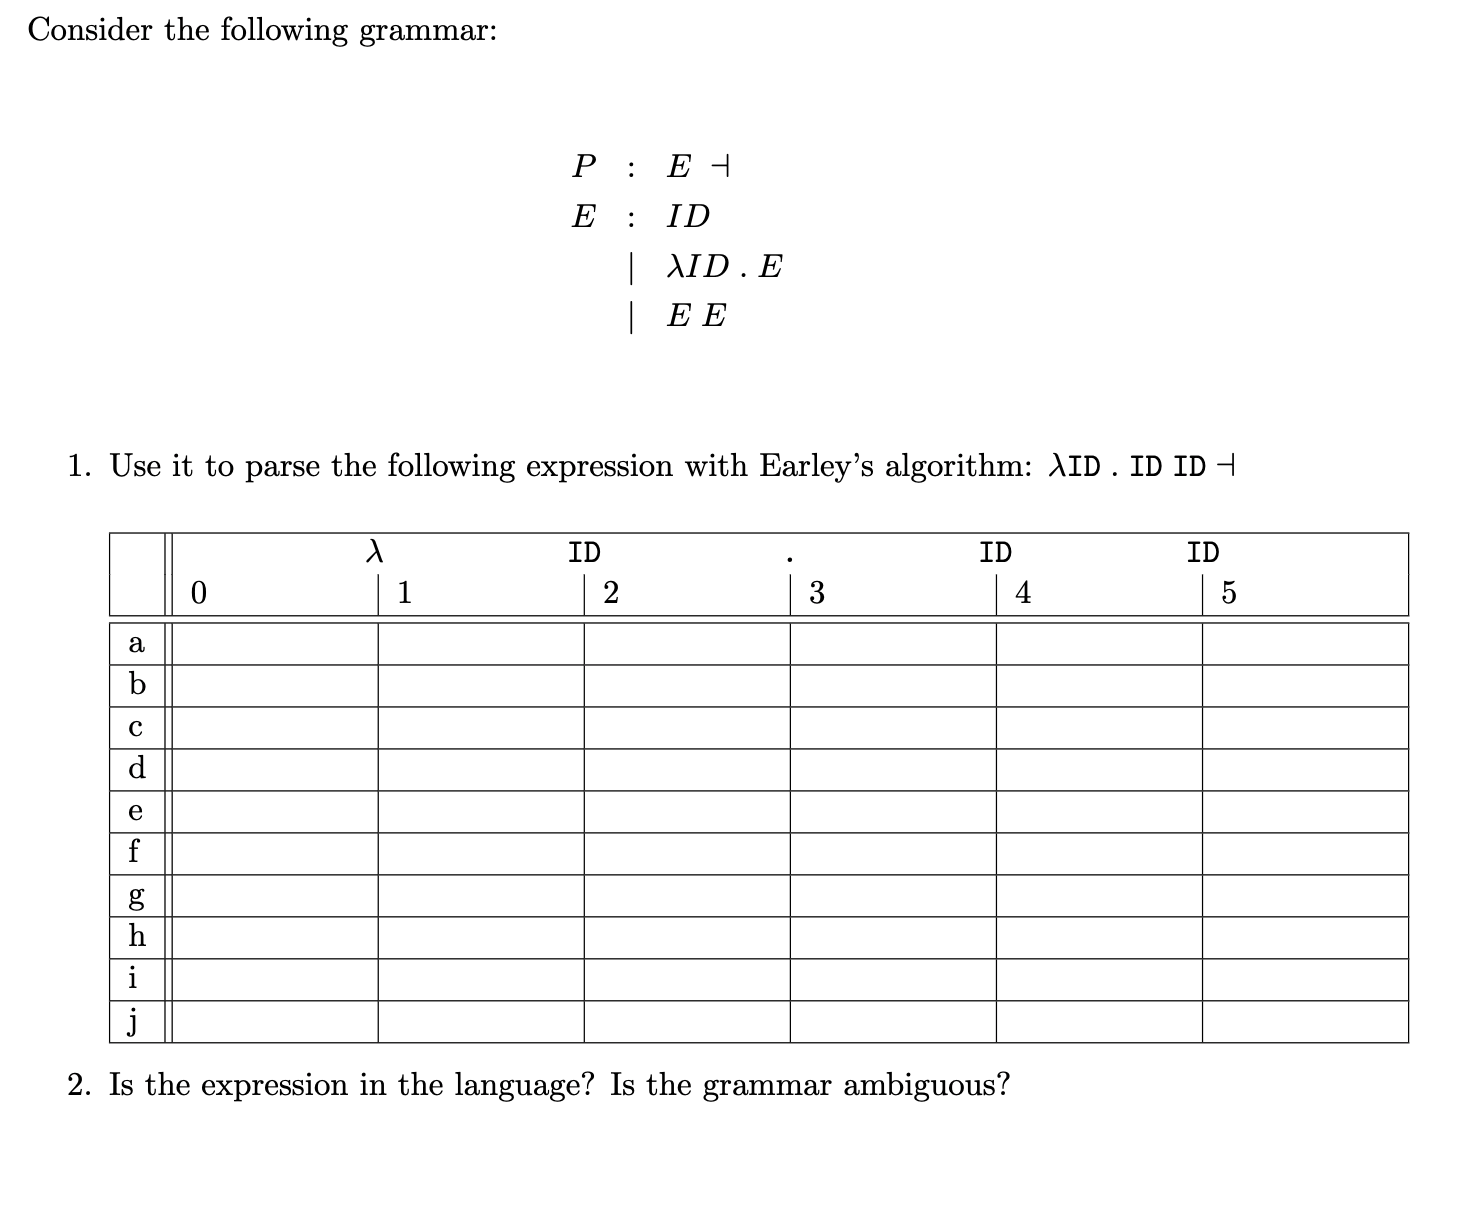
\includegraphics[height=12cm]{img/Snipaste_2021-04-12_17-39-39.png}
    \end{center}
    
\end{document}

